\documentclass[border=6pt]{standalone}
\usepackage{amsmath,amssymb}
\usepackage{tikz}
\usetikzlibrary{decorations.pathreplacing,calc,positioning}
% TikZ styles and helpers shared by figures/circuits.tex and figures/circuits_qsvt.tex
\tikzset{
  wire/.style={line width=0.55pt},
  gate/.style={draw,fill=white,minimum height=6.2mm,minimum width=7.5mm,inner sep=1.5pt,font=\small,line width=0.55pt},
  wgate/.style={gate,minimum width=13mm},
  ctrl/.style={circle,fill=black,inner sep=0pt,minimum size=1.9mm},
  octrl/.style={circle,draw,fill=white,inner sep=0pt,minimum size=1.9mm,line width=0.55pt},
  targ/.style={circle,draw,inner sep=0pt,minimum size=3.2mm,line width=0.55pt},
  meter/.style={draw,fill=white,minimum height=6.2mm,minimum width=7.5mm,line width=0.55pt},
  reg/.style={font=\small,anchor=east},
  blk/.style={font=\footnotesize,anchor=north,text=black!65},
  st/.style={font=\footnotesize,anchor=south,text=blue!45!black},
  brace/.style={decorate,decoration={brace,mirror,amplitude=2.2pt},line width=0.4pt,black!60},
  slash/.style={},
}
\newcommand{\slashwire}[3]{% x y label : the /n mark on a multi-qubit wire
  \draw[line width=0.7pt] (#1cm-1.3mm,#2cm-1.6mm) -- (#1cm+1.3mm,#2cm+1.6mm);
  \node[font=\scriptsize,anchor=south west,inner sep=0.4pt] at (#1cm+0.9mm,#2cm+0.9mm) {#3};}
\newcommand{\vsep}[3]{% x ybot ytop : a dashed block boundary
  \draw[dashed,black!45,line width=0.4pt] (#1cm,#2cm) -- (#1cm,#3cm);}


% box spanning wires: x, ytop, ybot, width(cm), label
\newcommand{\mb}[5]{\draw[fill=white,line width=0.55pt] (#1-#4/2,#2+0.31) rectangle (#1+#4/2,#3-0.31); \node[font=\small] at (#1,{(#2+#3)/2}) {#5};}
\newcommand{\gt}[3]{\node[gate] at (#1,#2) {#3};}
\newcommand{\wg}[4]{\node[gate,minimum width=#3] at (#1,#2) {#4};}
\newcommand{\ct}[2]{\node[ctrl] at (#1,#2) {};}
\newcommand{\oc}[2]{\node[octrl] at (#1,#2) {};}
\newcommand{\vl}[3]{\draw[wire] (#1,#2) -- (#1,#3);}
\newcommand{\tg}[2]{\node[targ] at (#1,#2) {}; \draw[wire] (#1,#2-0.16) -- (#1,#2+0.16);}
\newcommand{\meas}[2]{\node[meter] at (#1,#2) {}; \draw[wire] (#1-0.25,#2-0.12) arc (160:20:0.27); \draw[wire,-latex] (#1,#2-0.12) -- (#1+0.2,#2+0.12);}
\newcommand{\wires}[3]{\foreach \y in {#3} {\draw[wire] (#1,\y) -- (#2,\y);}}
\newcommand{\lab}[3]{\node[reg] at (#1,#2) {#3};}
\definecolor{hitp}{RGB}{118,68,160}
\definecolor{classic}{RGB}{90,90,90}
\newcommand{\cbox}[6]{\draw[rounded corners=3pt,fill=black!4,draw=black!45,line width=0.5pt] (#1,#2) rectangle (#3,#4); \node[font=\footnotesize,align=center,text width=#6] at ({(#1+#3)/2},{(#2+#4)/2}) {#5};}
\begin{document}

\newcommand{\stg}[3]{\draw[densely dashed,black!35] (#1,#2) -- (#1,-2.05); \node[st] at (#1,#2) {#3};}
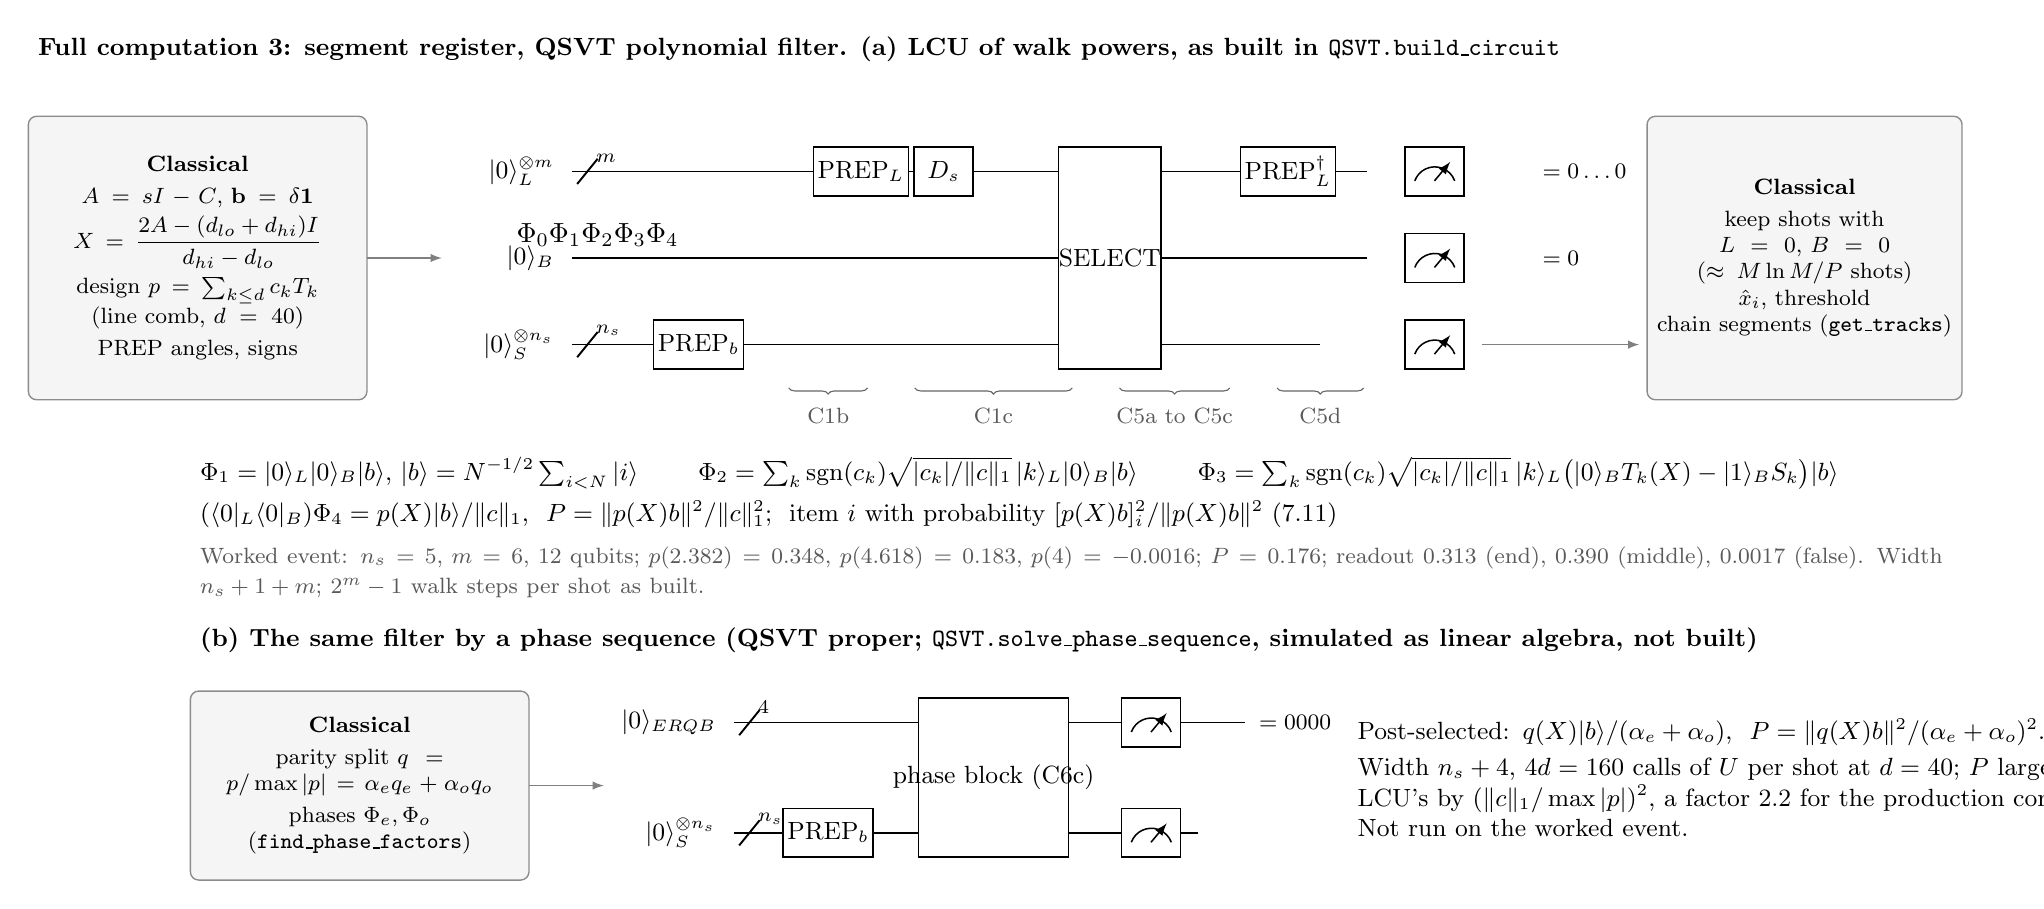
\begin{tikzpicture}[x=1cm,y=1cm]
\node[anchor=west,font=\small\bfseries] at (-6.2,2.45) {Full computation 3: segment register, QSVT polynomial filter. (a) LCU of walk powers, as built in \texttt{QSVT.build\_circuit}};
\cbox{-6.2}{1.6}{-1.9}{-2.0}{\textbf{Classical}\\[2pt] $A=sI-C$, $\mathbf b=\delta\mathbf 1$\\[2pt] $X=\dfrac{2A-(d_{lo}+d_{hi})I}{d_{hi}-d_{lo}}$\\[2pt] design $p=\sum_{k\le d}c_kT_k$\\ (line comb, $d=40$)\\[2pt] PREP angles, signs}{4.0cm}
\draw[-latex,black!50] (-1.9,-0.2) -- (-0.95,-0.2);
\lab{0.6}{0.9}{$|0\rangle^{\otimes m}_L$} \lab{0.6}{-0.2}{$|0\rangle_B$} \lab{0.6}{-1.3}{$|0\rangle^{\otimes n_s}_S$}
\wires{0.7}{10.8}{0.9,-0.2} \wires{0.7}{10.2}{-1.3} \slashwire{0.9}{0.9}{$m$} \slashwire{0.9}{-1.3}{$n_s$}
\stg{1.05}{1.35}{$\Phi_0$}
\wg{1.9}{-1.3}{11mm}{$\mathrm{PREP}_b$}
\stg{2.75}{1.35}{$\Phi_1$}
\wg{3.55}{0.9}{11mm}{$\mathrm{PREP}_L$} \gt{4.6}{0.9}{$D_s$}
\stg{5.25}{1.35}{$\Phi_2$}
\mb{6.3}{0.9}{-1.3}{1.3}{SELECT}
\stg{7.25}{1.35}{$\Phi_3$}
\wg{8.15}{0.9}{11mm}{$\mathrm{PREP}_L^\dagger$}
\stg{9.0}{1.35}{$\Phi_4$}
\meas{9.6}{0.9} \meas{9.6}{-0.2} \meas{9.6}{-1.3}
\node[font=\footnotesize,anchor=west] at (10.85,0.9) {$=0\ldots0$}; \node[font=\footnotesize,anchor=west] at (10.85,-0.2) {$=0$};
\draw[brace] (1.4,-1.85) -- (2.4,-1.85); \node[blk] at (1.9,-1.98) {C1b};
\draw[brace] (3.0,-1.85) -- (5.0,-1.85); \node[blk] at (4.0,-1.98) {C1c};
\draw[brace] (5.6,-1.85) -- (7.0,-1.85); \node[blk] at (6.3,-1.98) {C5a to C5c};
\draw[brace] (7.6,-1.85) -- (8.7,-1.85); \node[blk] at (8.15,-1.98) {C5d};
\draw[-latex,black!50] (10.2,-1.3) -- (12.2,-1.3);
\cbox{12.3}{1.6}{16.3}{-2.0}{\textbf{Classical}\\[2pt] keep shots with $L=0$, $B=0$\\ ($\approx M\ln M/P$ shots)\\ $\hat x_i$, threshold\\ chain segments (\texttt{get\_tracks})}{3.8cm}
\node[font=\small,anchor=north west,text width=22.5cm] at (-6.2,-2.6) {\raggedright
$\Phi_1=|0\rangle_L|0\rangle_B|b\rangle$, $|b\rangle=N^{-1/2}\sum_{i<N}|i\rangle$ \qquad
$\Phi_2=\sum_k\mathrm{sgn}(c_k)\sqrt{|c_k|/\lVert c\rVert_1}\,|k\rangle_L|0\rangle_B|b\rangle$ \qquad
$\Phi_3=\sum_k\mathrm{sgn}(c_k)\sqrt{|c_k|/\lVert c\rVert_1}\,|k\rangle_L\big(|0\rangle_BT_k(X)-|1\rangle_BS_k\big)|b\rangle$\\[4pt]
$(\langle0|_L\langle0|_B)\Phi_4=p(X)|b\rangle/\lVert c\rVert_1$, \ $P=\lVert p(X)b\rVert^2/\lVert c\rVert_1^2$; \ item $i$ with probability $[p(X)b]_i^2/\lVert p(X)b\rVert^2$ (7.11)\\[4pt]
\footnotesize\color{black!65} Worked event: $n_s=5$, $m=6$, 12 qubits; $p(2.382)=0.348$, $p(4.618)=0.183$, $p(4)=-0.0016$; $P=0.176$; readout 0.313 (end), 0.390 (middle), 0.0017 (false). Width $n_s+1+m$; $2^m-1$ walk steps per shot as built.};
% (b) phase sequence variant
\begin{scope}[shift={(0,-6.6)}]
\node[anchor=west,font=\small\bfseries] at (-6.2,1.55) {(b) The same filter by a phase sequence (QSVT proper; \texttt{QSVT.solve\_phase\_sequence}, simulated as linear algebra, not built)};
\cbox{-6.2}{0.9}{-1.9}{-1.5}{\textbf{Classical}\\[2pt] parity split $q=p/\max|p|=\alpha_eq_e+\alpha_oq_o$\\[2pt] phases $\Phi_e,\Phi_o$\\ (\texttt{find\_phase\_factors})}{4.0cm}
\draw[-latex,black!50] (-1.9,-0.3) -- (-0.95,-0.3);
\lab{0.6}{0.5}{$|0\rangle_{ERQB}$} \lab{0.6}{-0.9}{$|0\rangle^{\otimes n_s}_S$}
\wires{0.7}{7.2}{0.5} \wires{0.7}{6.6}{-0.9} \slashwire{0.9}{0.5}{$4$} \slashwire{0.9}{-0.9}{$n_s$}
\wg{1.9}{-0.9}{11mm}{$\mathrm{PREP}_b$}
\mb{4.0}{0.5}{-0.9}{1.9}{\small phase block (C6c)}
\meas{6.0}{0.5} \meas{6.0}{-0.9}
\node[font=\footnotesize,anchor=west] at (7.25,0.5) {$=0000$};
\node[font=\small,anchor=west,text width=10.3cm] at (8.5,-0.2) {\raggedright Post-selected: $q(X)|b\rangle/(\alpha_e+\alpha_o)$, \ $P=\lVert q(X)b\rVert^2/(\alpha_e+\alpha_o)^2$.\\[2pt] Width $n_s+4$, $4d=160$ calls of $U$ per shot at $d=40$; $P$ larger than the LCU's by $(\lVert c\rVert_1/\max|p|)^2$, a factor 2.2 for the production comb (7.4). Not run on the worked event.};
\end{scope}
\end{tikzpicture}
\end{document}
